% \documentclass{article}
% \usepackage[utf8]{inputenc}
% %\usepackage{algorithm2e}
% %\usepackage[linesnumbered]{algorithm2e}
% %\usepackage[linesnumbered,ruled]{algorithm2e}
% \usepackage[linesnumbered,ruled,vlined]{algorithm2e}
% \usepackage{graphicx}

\graphicspath{ {./images/} }

% \title{ Introducing realistic trading dynamics to the Bristol Stock Exchange}
% \author{Dhammatorn Riewcharoon (dr17549) supervised by Dr.John Cartildge }
% \date{February 2020}


% \begin{document}
% \tableofcontents{}
% \maketitle

% \section{Introduction}
\section{Contemporary Financial Market} 
The motivation of this project comes from the desire to understand and explore realism in simulating a contemporary financial stock market. When the first stock market was established, it was heavily reliant on human traders to offer a bid (buy order) and an ask (sell order) at specific price in order to create a market. However, the contemporary financial market has become heavily reliant on automated trading systems for transactions, which raises the question of how these so-called trading systems can dominate the market than one another. Because a change in price can happen in less than a second with 6.43 billion trades happening each day, it is nearly impossible for any human to keep up \cite{dailytrade}. In the years to come, more and more algorithmic traders will participate in the market. This change is inevitable and is now a common knowledge that no matter what we do, these trading systems will outperform human traders. It is commonly known in the U.S. that 80\% of the daily volume traded is executed by automated systems \cite{percentAgent}. There is no doubt this number will increase in the following years due to the fact that robot trader or ``autonomous agents” can work longer hours and require no salary to perform the same or even better than human traders. 

Over the last two decades, there has been a significant increase and interest in study of so called autonomous agents. With previous research from world renowned economist Vernon Smith who, in 1962, was able to prove that markets with limited unskilled participants was able to converge to an equilibrium point \cite{smith1962}. Through Smith’s style experiment, researchers were able to perform experiments on autonomous agents which includes ZI-C, ZI-P and Kaplan’s Sniper (explain in detail in Chapter 3). As these agents emerged, there has been an on-going study on their impact in a simulated market similar to Smith's experiments.  

By studying the behaviour of these agents, we now have a better insight on the impact of the agents in a market, more specifically in a simulated market where certain variables can be controlled. In previous literature, it has been proven that these agents' behaviour can alter when implemented in a market where an aspect of realistic market dynamics has been reinforced. This project will focus on an alternative method to introduce realism by implementing McG (shorthand for trading agents and model described in McGroarty et al.'s (2018) paper) \cite{McGroarty} agents in the Bristol Stock Exchange (BSE), a simple simulated financial market \cite{BSE_code}. 

\section{Terminologies of Order book types}
\subsection{Limit Order Book}
The majority of large financial markets now employ a Limit Order Book system, which can handle fast and effective trades in a matter of milliseconds. In a Limit Order Book system, a trader can submit either a buy (bid) or a sell (ask) with a specified price and a quantity. The Limit Order Book algorithm will then attempt to match a bid with another ask submitted with the price given. If there is no order on the other side of the book, the order will then sit on the list until it can be matched. 

\subsection{Limit Price}
In a Limit Order Book market, an agent can choose to submit a limit bid order or a limit ask order. This guarantees that the bid order will be executed at that price point or lower and the ask limit order will be executed at the price point or higher. However, because of the nature of the Limit Order Book, it is possible that the trade will never be executed since there is no guarantee that another order that can match this condition sits at the opposite of the book at any time. 

\subsection{Market Order}
A market order is similar to a Limit Order but does not care what the price is as long as the quantity is matched. When a market order is submitted to the Order Book, the algorithm will go through the opposite side of the book to match the order with another order like in a Limit Order book. However, if there are no orders on the other side, the market order will not be listed back on its own side, but reported as a failed attempt to trade back to the agent. If there is an order to match, the algorithm will make a match until the quantity is fulfilled, regardless of the price. 

\section{Experimental Economics}
The experiments conducted in this paper are based on what is called a Continuous Double Auction (CDA) market. In the market, the buyer is able to offer a price at any given time (commonly known as a bid) with an overall expectation that the price will increase over time. The seller, similarly, is also able to offer a price (commonly known as an ask)  at any given time, with a general market expectation that it will decrease over time. In addition, a buyer and a seller can accept the opposite’s offer at any given time, known as a trade. In the market, there is commonly a time limit in which the buyers and sellers are able to make such offers and trades, but both economic agents will be able to enter, exit or participate at any given point in the time period. CDA is highly common in the modern financial world, with stock markets, raw material market or cryptocurrency market employing a similar type. 

The development of experimental economics started in the 1960s with Vernon Smith, who performed a series of experiments with inexperienced (students) human traders to study competitive market behaviour in the CDA market. Smith’s goal was to analyze such market by reducing its complexity to understanding the mechanism with human traders. Smith’s 1962 experiment was conducted by dividing a group of participants into buyers who can only bid and sellers who can only ask \cite{smith1962}. These buyers are constrained to buy no more than their limit price and sellers sell at no lower than their limit price. Each session or ‘days’ run as buyers and sellers can ‘shout’ or submit an order to the market with a certain price. The opposite side can then accept or ignore the submitted order, in which a trade is being made. The trader will drop-out of the market when their unit/quantity runs out to zero or the time limit of each session is reached. 

Smith successfully showed that with remarkably low number of participants in the market with no experience of trading or finance can converge to the market competitive equilibrium. This implies to how agents do not need the full knowledge of demand and supply curve (price level at each quantity for the bid and ask side) in order to contribute to an allocatively efficient market \cite{smith1962}. In short, the allocative efficient point of a market is where the supply intersects the demand of the market. This is equivalent to the point where the demand of the market is equal to how much the producers can supply the products to the consumer. The questions researchers are asking after Smith’s experiment in later works is that, if limited knowledge human agents can participate in the market which converges to the equilibrium, how can we adapt or implement a similar an algorithmic agent to do the same. This paper marked the start of a new economics researching field called experimental economics and Smith’s 62 style of conducting the experiment became very relevant, 50 years later.

\section{Agent Based Model}
An agent based model (ABM) , like the BSE, consists of a market where agents can interact with one another. It may contain a homogeneous market (a market where all agents are of the same type) or in-homogeneous (contains different types of agents) similar to the market presented in McG's paper. In addition, an ABM can provide insight to the market overall, which represents the allocative efficiency and price equilibrium. In this paper, an agent based model is incredibly useful as we are comparing the performance of different agents at the same time as well as looking at the efficiency of the market and convergence towards equilibrium, much like Smith’s 62 experiment.

In a similar manner, Santa Fe Institute provided a simulated CDA market in order to study the interaction of robotic agents in which researchers could submit their version of these autonomous agents to compete for \$10,000 prize \cite{Santafe}. The winner of said competition is an agent called Sniper by Todd Kaplan (later known as Kaplan’s Sniper). The Kaplan’s Sniper algorithm strategy could be explained as sitting and waiting to “snipe” the best price, waiting either for the best spread (difference between the best bid and best offer) to fall to a small value, or the best offer is lower than the previous period’s smallest transaction price or until the current session is coming to an end. This algorithm, despite being very simple, was very effective. 

\subsection{Early development of Trading Agents}
Another similar Smith experiment was conducted in 1993, but this time with algorithmic trading agents called ZI-C (Zero-Intelligence Constrained) where similar results to that of Smith’s could be obtained  \cite{godesunder93}. Gode and Sunder were interested in understanding how much of CDA market equilibrium was affected from intelligence of agents and the organisation of market itself. Hence, they developed the so called ZI-C and ZI-U (Zero-Intelligence Unconstrained). The ZI-C is a simple algorithm that bids and asks at random prices but is constrained not to make a loss. By performing similar experiments with Smith’s 1962 \cite{smith1962} paper with both ZI-C and humans, they discovered that ZI-C results were surprisingly human-like and was able to converge at the equilibrium price at the end of each trading session. The result is remarkable because assumptions were made that some intelligence was needed for traders, both buyers and sellers in the market, in order to converge to the equilibrium which Gode and Sunder successfully shown that it is not the case. In addition, in 1994, Gode and Sunder provided evidence that ZI-C performance has a similar allocative efficiency of that of human agents. 

However, in 1997, Dave Cliff proved that ZI-C did not reach an equilibrium when certain conditions were met, which is when the price elasticity of supply and demand are different \cite{zip1997}. As a result, ZI-P (Zero-Intelligence Plus) was introduced and shown to outperform ZI-C in market conditions that failed. Unlike ZI-C, ZI-P was written so that the submitted price depended on not only the limit price, but also a margin coefficient. The main difference between ZI-C and ZI-P is that not only ZI-P is autonomous but also adaptive. Each individual ZI-P agents has the ability to alter the margin coefficient overtime, depending on the market. 

\subsection{Trading Agent Dominance}
Coming back to the recent years, there has been a debate over which algorithm dominates another in multiple papers. In this context, dominance indicates that the agent is better at generating profit in stock trading and a better loss-prevention decision system. The original claim by Das et al. sparked the search and development for such agents and gained massive industry attention \cite{das2001}. 

Again in 2006, Vytelingum claimed to have developed another agent Adaptive-Aggressive (AA) which beat ZI-P in a similar Smith-style experiment \cite{AA2006}. Then again in 2011 where it is shown to dominate against GDX \cite{deluca2011}. In many cases, AA is beaten by ZI-P and GDX. These papers demonstrate how the dominance of said agents are subject to homogeneous and Smith style experiments which often overlooks the importance of realism in the market. The aim of this thesis is to introduce an alternative way of introducing realism in order to investigate the impact of these agents on the market. 

\section{Simulating a realistic market}
As mentioned, because the previous experiments that were conducted with the trading agents which claimed dominance over one another was done in a non-realistic environment. This raised doubts about how well the agents will actually perform in a more realistic market. There have been papers that explored the concept of realism in the past. 

Das et al. (2001) \cite{das2001} also explored this concept of latency in which agents would sleep and wake at a different cycle. In the slow cycle, in addition to 5 second of sleep time, agents would wake up only on trades. In the fast cycle, agents would sleep for 1 second and wake up on all orders and trades. This illustrates the approach to mimic realism in financial market as human agents wouldn’t be able to look at every changes in order and trades. 

In a recent study by Hanifan and Cartildge (2019) \cite{foolsrush} explored the concept of reaction time in a modelled market. This includes so-called communication latency and trading latency. Evidently, the study demonstrated that adaptive algorithms such as AA and ZI-P, when a certain aspect of realism is introduced, the dominance of said algorithms decreases and simpler algorithm prevails. 

On the same note, Cliff (2019) illustrated that MAA (Modified AA) does not dominate in a simulated real world market in which the underlying equilibrium price was varied dynamically. AA hugely underperformed by ZI-P. The importance is then again emphasized as Cliff described ``AA’s success as reported in previous papers is largely due to the extent to which its internal mechanisms are designed to fit exactly the kind of experiment settings first introduced by Vernon Smith” (Cliff 2019, p.13) \cite{dcliff2013}. 

\section{Bristol Stock Exchange (BSE)}
Professor Dave Cliff, in 2018, presented a market stock exchange simulator called Bristol Stock Exchange designed for university-level study of algorithmic behaviour of trader agents and stock market in general implemented in Python \cite{BSE_code}. The simulator is a full implementation of the Limit Order Book system which accepts a limit order or quotes from each agent. A limit order can either be a bid (buying) or an ask (selling). The BSE divides the LOB into 2 sides, a bid and an ask, in which quotes from each side is listed. The matching and trading process is the same as described in the Limit Order Book. To process an ask order in the BSE(Bristol Stock Exchange), the Limit Order Book system will, first match the ask order with the first bid order in a sorted list with the highest price, then while the highest bid is higher than the best ask price, it will go down the list until all the quantity of the given ask order is complete. If there is not enough bid orders, the ask order will be posted back to the Limit Order ask side of the Book and vice versa for processing a bid order.

The BSE interacts with each agent in a time step manner. In each time step, the system randomly chooses an agent from a list of both buyers and sellers. The agent can then choose to submit an order or wait for another round. At the end of each timestep, the agent update their own internal status. In the current version, the BSE only accepts a limit order with a quantity of 1 at a certain price. In order to correctly implement McG’s agents, accepting different quantities at different price must be implemented. Similarly, for a market order, the BSE will go down the opposite side of the book until the quantity is fulfilled regardless of the price.

\section{McG's approach on realism}
As seen in the section 1.5, there has been attempts to implement some form or element of realism to the environment of the agents. However, McG claims that their model is ``realistic and robust enough for the analysis of algorithmic trading strategies"\cite{McGroarty} in which the McG agents represents the most common strategies and behaviour found in the real financial exchange. In this manner, the model is a better replication of price movement in the real financial exchange. 

McG describe their approach of creating realism by grouping different strategies of traders in the real market into 5 basic agents : Market maker, Liquidity consumers, Momentum traders, Mean reversion traders and Noise traders. McG then divide the time-steps in which agent can execute their order into 300,000 time steps per trading period which is derived from 8.5hr trading day period divided into 10th of a second. The McG selection of agent and timing system will be called ``action-step" in order to avoid confusion with the BSE's time-step system. In each action-step, the agent has a certain probability to act, represented by the symbol $\delta$. If the agent chooses to act, it can choose to submit a new order, cancel an order or update its internal status. According to McG, this implementation of the simulated time is closer to how traders reacts with the change in price of the market compared to randomly choosing an agent in each time-step is unrealistic. In addition, the agent can choose not to act and only update its own internal status.

\section{Extreme Price Event}
One feature of the realistic dynamics presented in McG is extreme price events which can be seen in real financial market, more specifically, \textbf{Price Spikes}. McG defines their price spike the same as Johnson et al. which is  defined as ``an occurrence of the stock price ticking down (or up) at least ten times before ticking up (or down) and the price change exceeding 0.8\% of the initial price" \cite{Johnson}. Johnson et al. reported as high as 18,520 crashes in the market between January 3rd 2006 and February 3rd 2011 in various stocks with duration less than 1500 ms. Since the introduction of trading agents and ultrafast trading dynamics, these ultrafast extreme events (UEE) are more prevalent and thus, highlights the need to understand this new dynamic. 

\begin{figure}[h]
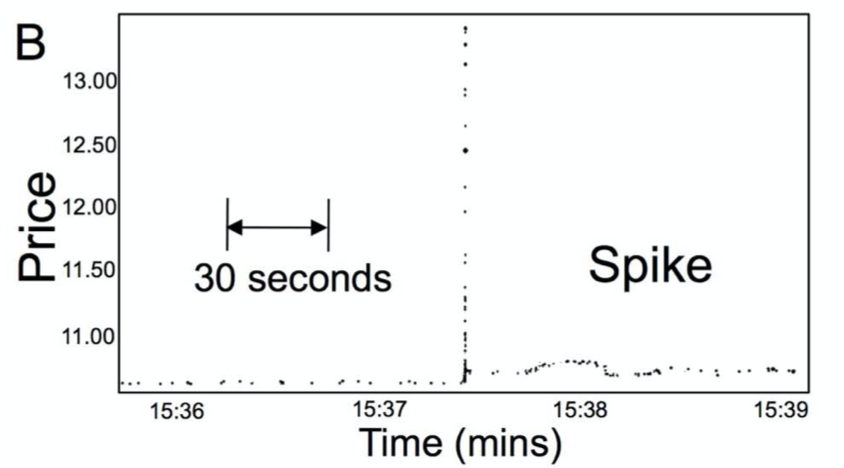
\includegraphics[ height=8cm]{Dissertation/images/Background/johnson price spike.png}
\caption{Price Spike example reproduced from \cite{Johnson}}  
\end{figure} 
\FloatBarrier

The UEE duration is defined as the time period between the first tick and last tick in a certain direction of the price of an UEE event. Johnson et al. shows that these UEE durations generally fall below the human reaction time. In addition, the faster the UEE duration is, the more they become prevalent in the market. This illustrates how the UEE is unlikely to be originate from human traders. 

The reason why the study of these price events is becoming more important is because it can cause large swings in price and affects a firm's assets and value in the market. One example is the crash of an exchange operator called BATS after its IPO on 23rd March 2012. The initial price of the stock is \$15.25 and within 1.5ms the price fell to \$0.0007. BATS then later withdraw their IPO and reported a technical fault due to their high-speed trading algorithm bug. This causes investors and company that has made over \$100 million to return their earnings \cite{BATS}. This is not a single unique event but one of many that has happended in the last decade due to errors in the high-speed trading algorithms. The study of these so-called agents are therefore more important than ever in order to properly regulate the use of these agents and prevent such disaster from happening in the future. 



